\clearemptydoublepage
\chapter{Résultats \& Discussion}

\section{Résultats}



\section{Discussion}
\subsection{Un treillis en mémoire ?}
Comme nous l'avons vu dans la partie~\ref{conception_memoire_semantique} (page \pageref{conception_memoire_semantique}), la mémoire sémantique entrepose une matrice de booléens associant des formes remarquables à des plateaux. Ces associations correspondent typiquement à la définition d'un contexte, permettant la construction d'un treillis de concepts.

\subsubsection{Analyse de concepts formels}
FCA\footnote{Formal Concept Analysis (en Français \og Analyse de Concepts Formels \fg{}).} est l'étude de concepts définis de manière formelle, via un contexte. Cette section ne présente pas en détail FCA. Pour plus d'informations sur cette méthode d'analyse et les treillis de Galois nous vous recommandons la lecture des cours de Marianne Huchard et de Michel Liquière\footnote{Cours de Marianne Huchard, Professeur en informatique à l'université Montpellier 2 (Faculté des Sciences) et Directrice adjointe du LIRMM (Laboratoire d'Informatique, de Robotique et de Microélectronique de Montpellier) et de Michel Liquière, Maitre de Conférences dans la même université, disponibles à l'adresse suivante : \texttt{http://www.lirmm.fr/\textasciitilde huchard/Huchard/teaching.html}}.

\paragraph{Le contexte} Il s'agit d'un triplet $(G,M,I)$ avec $G$ et $M$ des ensembles et $I\subseteq G \times M$ des relations de $G$ dans $M$. Les éléments contenus dans $G$ sont appelés \emph{objets} et ceux de $M$ \emph{attributs}. $I$ est une relation entre une object de $G$ et un attribut de $M$, et qui se dit \og l'objet $g$ possède l'attribut $m$ \fg{}. (Source : Wikpiedia\footnote{L'article \og Analyse de concepts formels \fg{} de Wikipedia en Français à considérablement aidé à la rédaction de cette partie. Contenu sous licence CC-BY-SA.})

En application à \cogito{} nous aurions :

\begin{tabular}{r c l}
$G$ & $ = $ & ensemble des plateaux (objets),\\
$M$ & $ = $ & ensemble des formes remarquables (attributs),\\
$I$ & $ = $ & ensemble des relations plateaux / formes remarquables\\
& & définies dans la matrice actuelle.\\
\end{tabular}

Construire des concepts à partir du contexte formel permettrait de raisonner à un niveau d'abstraction supplémentaire. Actuellement \cogito{} travail sur des formes remarquables, après la construction d'un treillis de Galois, il pourrait raisonner sur des ensembles de formes remarquables.

\paragraph{Et concrètement ?}Prenons un exemple simple et parlant pour la plupart des passionnés d'informatique\footnote{Alias \og Nerd \fg{}.} : 

\begin{minipage}[c]{0.5\textwidth}
\centering
Nous aimons le \textbf{café} \\ 

\includegraphics[width=0.6\textwidth]{files/conclusion/espresso} \\
Situation \emph{café}
\end{minipage}
\begin{minipage}[c]{0.5\textwidth}
\centering
Nous adorons l'\textbf{ordinateur} \\ 

\includegraphics[width=0.6\textwidth]{files/conclusion/ordi} \\
Situation \emph{ordinateur}
\end{minipage}

\begin{center}
En revanche nous n'apprécions pas le café à proximité de l'ordinateur.
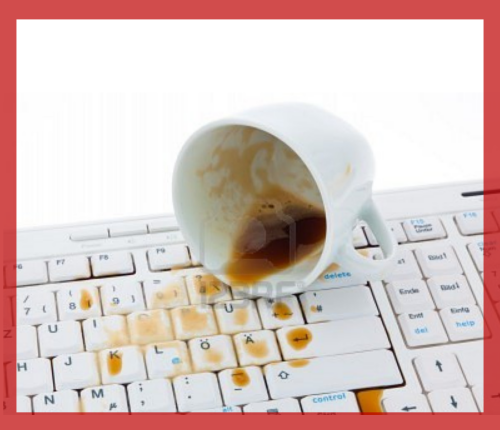
\includegraphics[width=0.6\textwidth]{files/conclusion/cafe_renverse} \\
Situation \emph{café renversé sur l'ordinateur}
\end{center}

Le modèle \cogito{} actuel raisonnerait distinctement sur le \emph{café} et sur l'\emph{ordinateur}, qui seraient des attributs. Lors de la rencontre de la situation \emph{café renversé sur l'ordinateur}, les valeur des attributs \emph{café} et \emph{ordinateur} seraient donc diminués. Avec la construction d'un treillis de Galois, il serait possible de dévaloriser le concept regroupant les deux attributs \emph{café} et \emph{ordinateur}, sans nuire aux concepts qui ne sont composé que d'un des deux attributs.